Монады в Yesod

Как вы уже увидели, в этой книге появилось несколько монад: Handler, Widget и YesodDB (для Persistant). Как и всякая монада, каждая из них предоставляет некоторую специфическцю функциональность: Handler предоставляет доступ к запросу и позволяет отправлять ответы, Widget содержит HTML, CSS и Javascript, а YesodDB позволяет делать запросы к базе данных. В терминах Model-View-Controller (MVC), мы могли бы рассматривать YesodDB как модель, Widget как представление, и Handler как контроллер.

До сих пор у нас были представлены очень простые способы использования этих монад: основной обработчик работает в монаде Handler, используя runDB для выполнения запроса в YesodDB и defaultLayout для возврата монады Widget, которая в свою очередь была создана вызовом toWidget.

Тем не менее, если у нас будет глубокое понимание этих типов, мы сможем достичь более интересных результатов.

Трансформаторы Монад

Монады они как луковицы. Монады не как пироженные. Вроде бы Шрек.

Прежде чем мы углубимся в монады Yesod, мы должны немного понимать трансформаторы монад. (Если вы уже знаете о трансформаторах монад всё, вы, скорее всего, можете пропустить этот раздел.) Различные монады предоставляют различную функциональность: Reader предоставляет доступ только для чтения к некоторым данных по всему вычислению, Error позволяет оборвать вычисления, и так далее.

Однако, часто вы захотите иметь возможность объединить функциональные возможности некоторых из этих монад. В конце концов, почему бы не иметь вычисление с доступом только для чтения к некоторым параметрам настройки, которое в любой момент могло бы прерваться с ошибкой? Одним из подходов было бы написать новую монаду, например ReaderError, но это имеет очевидный недостаток экспоненциальной сложности: будет нужно писать новую монаду для каждой возможной комбинации.

Вместо этого мы используем трансформаторы монад. Вместе с Reader, у нас есть ReaderT, который добавляет функциональность Reader к любой другой монаде. Таким образом, мы могли бы представить ReaderError как (концептуально):

\begin{lstlisting}
type ReaderError = ReaderT Error
\end{lstlisting}

Чтобы получить доступ к параметрам настройки, мы можем использовать функцию ask. А что насчет обрывания вычисления? Мы бы хотели вызвать throwError, но это не вполне будет работать. Вместо этого мы должны использовать lift, что бы втянуть наш вызов в монаду на уровень выше. Другими словами:

\begin{lstlisting}
throwError :: errValue -> Error
lift . throwError :: errValue -> ReaderT Error
\end{lstlisting}

Сейчас вы должны уловить несколько идей:

* Трансформатор может быть использован для добавления функциональных возможностей в существующие монады.
* Трансформатор должен всегда обертываться вокруг существующей монады.
* Функциональные возможности получившейся монады будут зависеть не только от трансформатора монады, но и от монады обёрнутой внутри.

Отличный пример для последнего утверждения это монада IO. Независимо от того, сколько слоев трансформаторов у вас есть вокруг IO, там всё ещё есть ядро IO, то есть вы можете выполнять I/O в любом из этих стеков трансформаторов монад. Вы будете часто видеть код, который выглядит как \lstinline'liftIO $ putStrLn "Hello There!"'.

Три Трансформатора

Мы уже обсуждали два наших трансформатора ранее: Handler и Widget. Просто напомним, есть два особенных факта об этих трансформаторов:

1) В целях упрощения сообщений об ошибках, они не являются фактическими трансформаторами. Вместо этого, они являются новыми типами (newtypes) с реализацией своей внутренней монады. Помните, что именно поэтому Yesod предоставляет специальную функцию lift, которая работает для Handler и Widget.
2) На самом деле у них есть дополнительные параметры типа для дополнительного и основного сайта. В результате, библиотеки Yesod предоставляют \lstinline'GHandler sub master a' и \lstinline'GWidget sub master a', и каждый сайт получает пару синонимов типов \lstinline'type Handler = GHandler MyApp MyApp' и \lstinline'type Widget = GWidget MyApp MyApp ()'.

В пакете Persistent, у есть класс типов который называется PersistStore. Этот класс типов определяет все примитивные операции которые можно выполнять с базой данных, к примеру получить данные (get). Этот класс типов по существу выглядит как \lstinline'class (Monad (Ь m)) => PersistStore b m'. Где b определяет сервер базы данных, а на самом деле является трансформатором монады, а m являеся внутренней монадой которую b оборачивает. И SQL и MongoDB имеют свои собственные экземпляры; в случае SQL, он выглядит так:

\begin{lstlisting}
instance MonadBaseControl IO m => PersistBackend SqlPersist m
\end{lstlisting}

Это означает, что вы можете работать с базой данных SQL с любой основной монадой, до тех пор пока эта монада поддерживает MonadBaseControl IO, что позволяет правильно обрабатывать исключения в стеке монад. В общем это означает означает любой стек трансформаторов построеный вокруг IO (кроме исключительных случаев, как ContT). К счастью для нас, это включает в себя как Handler так и Widget. Следовательно мы можем наслаивать наш Persistent трансформатор на Handler или Widget.

Это не всегда было так. Перед Yesod 0.10, Yesod был построен на базе пакета enumerators, который не поддерживает MonadBaseControl. В Yesod 0.10, мы перешли к пакету conduit, который значительно упрощает всё, что мы здесь обсуждаем.

Для того, чтобы упростить обращение к соответствующим Persistent трансформаторам, пакет yesod-persistent определяет ассоциированный тип YesodPersistBackend. Например, если у нас есть сайт который назвается MyApp и использует SQL, мы можем определить что-то вроде \lstinline'type instance YesodPersistBackend MyApp = SqlPersist'.

Когда мы захотим выполнить наши действия с базой данных, у нас будет SqlPersist обернутый вокруг Handler или Widget. Так мы cможем использовать стандартные функции развертки Persistent (например, runSqlPool) для исполнения действия и возврата в нормальный Handler/Widget. Для автоматизации этого, предоставляется функция runDB. Суммируя все это, мы теперь можем исполнять действия с базой данных внутри нашых обработчиков и виджетов.

Большую часть времени в коде Yesod, особенно до сих пор, виджеты рассматривались как контейнеры без возможности действий, которые просто объединяют вместе HTML, CSS и Javascript. Но если вы посмотрите на последний абзац еще раз, вы поймете, что это не совсем так. Поскольку виджет это трансформатор над обработчиком, всё что вы делаете в обработчике может быть сделано в виджете, в том числе и операции с базой данных. Все, что вам нужно сделать, это протянуть вызов используя lift.

Пример: Навигационная панель на основе базы данных.

Давайте применим некоторые из новых знаний на практике. Мы хотим создать Widget, который генерирует свой вывод на основе содержимого базы данных. Ранее мы бы загрузили данные в Handler, а затем передали эти данные в Widget. Теперь загрузим данные в самом Widget. Это хорошо для модульности, так как этот Widget cможет использоваться в любом Handler, каком мы захотим, без необходимости передавать содержимое базы данных.

\begin{lstlisting}
{-# LANGUAGE OverloadedStrings, TypeFamilies, TemplateHaskell, FlexibleContexts,
             QuasiQuotes, TypeFamilies, MultiParamTypeClasses, GADTs #-}
import Yesod
import Database.Persist.Sqlite
import Data.Text (Text)
import Data.Time

share [mkPersist sqlSettings, mkMigrate "migrateAll"] [persist|
Link
    title Text
    url Text
    added UTCTime
|]

data LinksExample = LinksExample ConnectionPool

mkYesod "LinksExample" [parseRoutes|
/ RootR GET
/add-link AddLinkR POST
|]

instance Yesod LinksExample

instance RenderMessage LinksExample FormMessage where
    renderMessage _ _ = defaultFormMessage

instance YesodPersist LinksExample where
    type YesodPersistBackend LinksExample = SqlPersist
    runDB db = do
        LinksExample pool <- getYesod
        runSqlPool db pool

getRootR :: Handler RepHtml
getRootR = defaultLayout [whamlet|
<form method=post action=@{AddLinkR}>
    <p>
        Add a new link to #
        <input type=url name=url value=http://>
        \ titled #
        <input type=text name=title>
        \ #
        <input type=submit value="Add link">
<h2>Existing links
^{existingLinks}
|]

existingLinks :: Widget
existingLinks = do
    links <- lift $ runDB $ selectList [] [LimitTo 5, Desc LinkAdded]
    [whamlet|
<ul>
    $forall Entity _ link <- links
        <li>
            <a href=#{linkUrl link}>#{linkTitle link}
|]

postAddLinkR :: Handler ()
postAddLinkR = do
    url <- runInputPost $ ireq urlField "url"
    title <- runInputPost $ ireq textField "title"
    now <- liftIO getCurrentTime
    runDB $ insert $ Link title url now
    setMessage "Link added"
    redirect RootR

main :: IO ()
main = withSqlitePool "links.db3" 10 $ \pool -> do
    runSqlPool (runMigration migrateAll) pool
    warpDebug 3000 $ LinksExample pool
\end{lstlisting}

В частности обратите внимание на функцию existingLinks. Видете, что всё, что нужно сделать, это применить lift к нормальному действию с базой данных. А в getRootR, мы трактуем existingLinks как обычный Widget, вообще без никаких специальных параметров. Смотрите на рисунке вывод этого приложения.

\begin{figure}[tbh]
  \centering
  \caption{Скриншот панели навигации}
  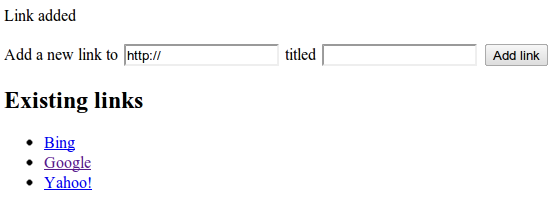
\includegraphics{13-yesods-monads-image-01.png}
\end{figure}

Пример: Запрос информации

Таким же образом вы можете получить информацию по звпросу внутри Widget. В этом примере мы определяем порядок сортировки списка на основе GET параметров.

\begin{lstlisting}
{-# LANGUAGE OverloadedStrings, TypeFamilies, TemplateHaskell,
             QuasiQuotes, TypeFamilies, MultiParamTypeClasses, GADTs #-}
import Yesod
import Data.Text (Text)
import Data.List (sortBy)
import Data.Ord (comparing)

data Person = Person
    { personName :: Text
    , personAge :: Int
    }

people :: [Person]
people =
    [ Person "Miriam" 25
    , Person "Eliezer" 3
    , Person "Michael" 26
    , Person "Gavriella" 1
    ]

data People = People

mkYesod "People" [parseRoutes|
/ RootR GET
|]

instance Yesod People

instance RenderMessage People FormMessage where
    renderMessage _ _ = defaultFormMessage


getRootR :: Handler RepHtml
getRootR = defaultLayout [whamlet|
<p>
    <a href="?sort=name">Sort by name
    \ | #
    <a href="?sort=age">Sort by age
    \ | #
    <a href="?">No sort
^{showPeople}
|]

showPeople :: Widget
showPeople = do
    msort <- lift $ runInputGet $ iopt textField "sort"
    let people' =
            case msort of
                Just "name" -> sortBy (comparing personName) people
                Just "age"  -> sortBy (comparing personAge)  people
                _           -> people
    [whamlet|
<dl>
    $forall person <- people'
        <dt>#{personName person}
        <dd>#{show $ personAge person}
|]

main :: IO ()
main = warpDebug 3000 People
\end{lstlisting}

Повторим, всё что нужно сделать, это протянуть функцию стандартную для Handler (в данном случае, runInputGet), чтобы исполнить её в нашем Widget.

Выводы

Если вы полностью проигнорировали эту главу, вы все равно сможете с большой пользой использовать Yesod. Преимущество понимания того, как взаимодействуют монады Yesod, в том, чтобы иметь возможность производить более чистый, и более модульный код. Способность выполнять произвольные действия в Widget может быть мощным инструментом, и понимание того, как взаимодействуют Persistent и ваш Handler код может помочь вам сделать более обоснованные проектные решения в вашем приложении.
